\chapter{电磁学与电动力学}
本章是以Maxwell方程组为核心来组织的。

\section{基本物理量与概念}
\subsection{电}
\subsubsection{电荷}
\paragraph*{物理对象}如下图所示为一些基本对象:
\begin{center}
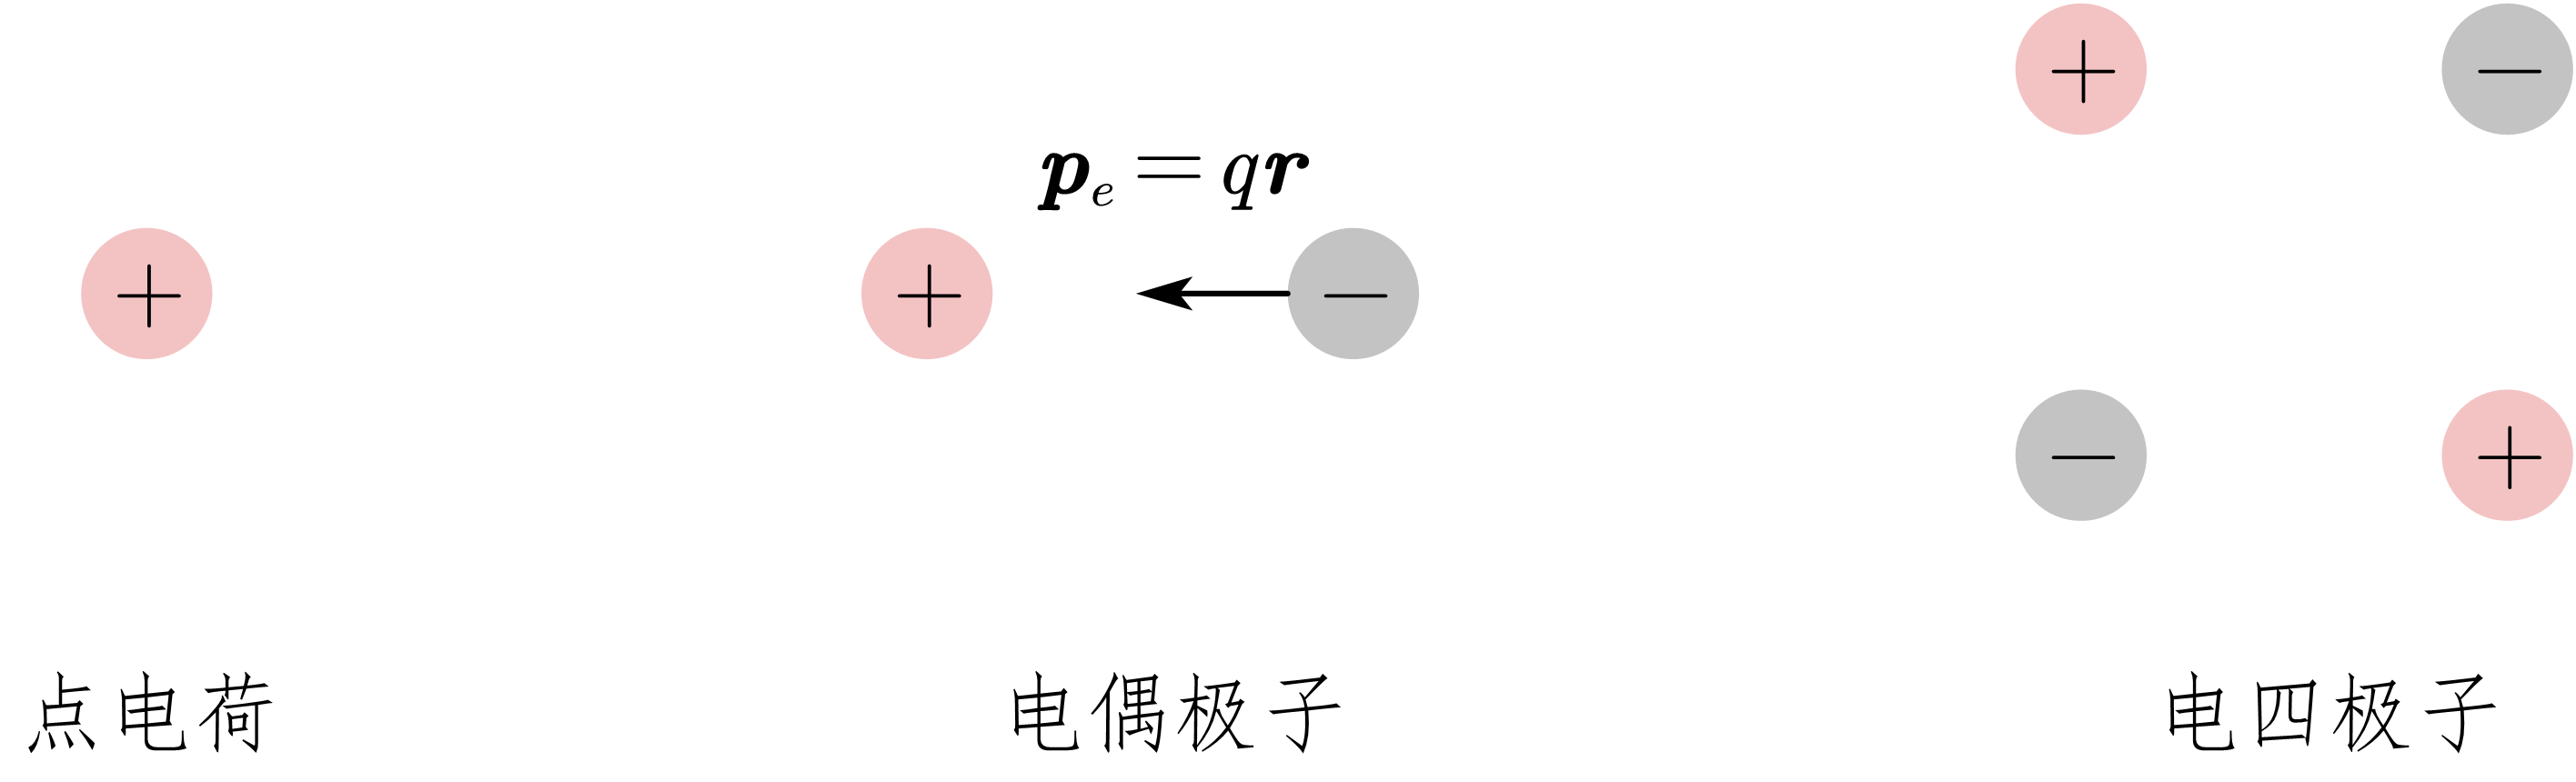
\includegraphics[width=10cm]{figure/ele-dyna-elec.png}
\label{charge-illustration}
\end{center}
\paragraph*{物理量}
\begin{description}
\item[电荷] 电荷$q$是基本粒子的基本属性.它是量子化的,即一个带电体的电荷是基本电荷电量的\qty{1.60217733e-19}{\coulomb}.夸克具有分数电荷$\pm\frac{1}{e},\pm\frac{2}{3}e$,但仍是量子化的。
\item[电荷体密度] 电荷分布在带电体上的密度,单位\si{\coulomb\per\cubic\m}:
\begin{empheq}{equation}
\rho=\odv{q}{v}
\end{empheq}
\item[电荷面密度] 电荷分布在曲面上的密度,单位\si{\coulomb\per\square\m}:
\begin{empheq}{equation}
\rho=\odv{q}{s}
\end{empheq}
\item[真空电容率] 国际单位制下为$q$\,\si{\ampere}电流在\qty{1}{\s}内累积的电荷量,也叫真空介电常数。表示为
$$\varepsilon_0=\SI{8.85e-12}{\square\coulomb\per(\newton\square\m)}$$
有时记$k=\inv{4\pi\varepsilon_0}$。
或者\si{\N\m}。
\item[偶极矩] 即之前图中的$\bm{p}_e$,一个电偶极子由偶极矩表示。
\end{description}
\subsubsection{电场}
\paragraph*{电场强度} 是一个矢量,表示为$\bE$。其大小的含义是单位正电荷在该点处所受的电场力的大小,其方向就是受力的方向。单位为\si{N\per\coulomb}。

与电场强度相关的概念有:
\begin{description}
\item[电通量] 是电场强度的曲面积分,标量:
$$\Phi_e=\iint_S \bE\cdot\dif s$$
其中$\dif s$为面片的单位元。
\item[电位移矢量] 用符号$\bm{D}$表示:
$$\bm{D}=\varepsilon_0\bm{E}+\bm{P}$$
单位\si{\coulomb\per\square\m}。对于线性各向同性的介质,有$\bm{D}=\varepsilon \bm{E}$,$\varepsilon$为电介质的绝对介电常数。电位移矢量的导数有以下表达式:
$$\pdv{\bm{D}}{t}=\nabla\times \bm{H}-\bm{J}$$
对应Maxwell方程\ref{maxwell-4}。
\item[电位移通量] 电位移矢量的曲面积分,是标量:
$$\Phi_{\bm{D}}=\iint_S\bm{D}\cdot\dif s$$ 
\item[点电荷的电场强度] 值为$\bE=k\frac{q}{r^3}\bm{r}$。它取绝对值就是$k\frac{q}{r^2}$,但是注意矢量可以叠加,但取绝对值之后不可叠加。
\end{description}
\paragraph*{电势}电场的基本属性,属于标量。含义是在某点$\bm{p}$移动1单位正电荷到零电势点$\bm{p}_0$时电场力做的功:
$$U(\bm{p})=\frac{W}{q}=\int_{\bm{p}}^{\bm{p}_0}\bE\cdot\dif \bm{l}$$
$\bm{l}$为积分路径。当电荷分布在有限区域内时,通常选择无穷远点为零电势点,则积分上界为$\infty$。电势在有的地方也用$\varphi$表示,$U$在电路中经常用来表示电压,即电势的差值。

对于静电场,电势与电场强度的关系为:
$$\bE=-\nabla U$$
由于$\vdiv \bE=0$,因此可以得到电势的拉普拉斯方程:
$$\Delta \varphi=0$$

由电势衍生出以下一些概念:
\begin{description}
\item[电势能] 电荷与电场的相互作用能。移动$q$电荷到零势能点所做的功:
$$W(\bm{p})=\int_{\bm{p}}^{\bm{p}_0}q\bE\cdot\dif \bm{l}$$
\item[点电荷的电势] 点电荷生成的电势为$U=\inv{4\pi\varepsilon_0}\frac{q}{r}$。
\item[偶极矩] 给定一个电荷体系,任取其中一个电荷为原点,则每个电荷具有径矢$\bm{r}_a$,现在考虑一个径矢为$\bm{R}_0$的点,则它的电势为:
$$\varphi=\sum \frac{q_i}{|\bm{R}_0-\bm{r}_i|}$$
这里省略系数$\inv{4\pi\varepsilon_0}$。如下图所示:
\begin{center}
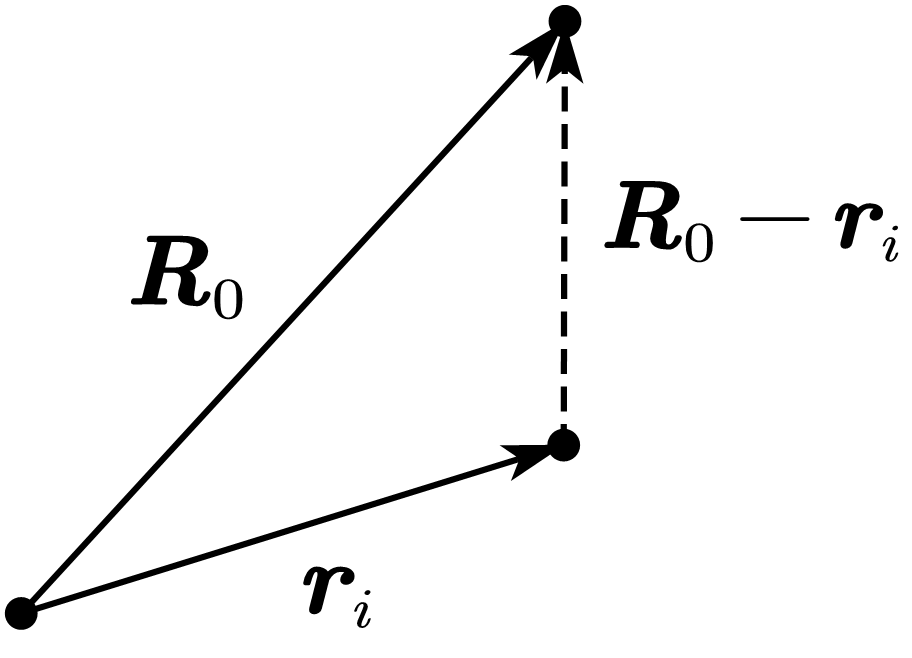
\includegraphics[width=4cm]{figure/elec-mag-single-point-charge-u.png}
\end{center}

当$\bm{R}_0\gg \bm{r}_i$时,把势函数在$\bm{R}_0$处展开:
\begin{empheq}{align}
\varphi=\frac{\sum q_i}{R_0}-\sum e_i \bm{r}_i\cdot \nabla \inv{R_0}
\end{empheq}
以上结论是通过取$f(\bx)=\sum \frac{q_i}{|\bx|}$,对它用一阶近似得到的。于是取
$$\bm{d}=\sum q_i\bm{r}_i$$
为电荷体系的偶极矩。

当$\sum q_i=0$时,偶极矩与坐标无关。同时,有该电荷体系在远距离处的电势为:
$$\phi=-\bm{d}\cdot\nabla\frac{1}{R_0}=\frac{\bm{d}\cdot \bm{R}_0}{R_0^3}$$
电场强度为
$$\bE=-\nabla \frac{\bm{d}\cdot\bm{R}_0}{R_0^3}=-\inv{R_0^3}\nabla (\bm{d}\cdot\bm{R}_0)-(\bm{d}\cdot\bm{R}_0)\nabla \inv{R_0^3}$$


对于图\ref{charge-illustration}中的电偶极子,偶极矩就是$\bm{d}=q\bm{r}$,取绝对值$d=qr$,这时与一般的定义一致。这里$\bm{r}$是从负电荷指向正电荷的径矢。
\end{description}

\subsubsection{电介质}
\paragraph*{带电荷导体的静电场}一个带电荷导体具有静电场,在静电平衡时,其内部的场强必然为0,否则引起电荷运动。因此平衡时电荷应该分布在导体的表面,且导体表面的电场强度应该垂直于表面,或切向分量为0:
$$\bE_t=\bm{0}$$
否则引起电荷在切向的运动。由于$\bE=-\nabla \varphi$,因此导体在表面的电势应当相同。

根据$\vdiv \bE=4\pi\bar{\rho}$,$\bar{\rho}$为平均电荷密度。可得$E_{\bn}=4\pi\sigma$,$\sigma$为电荷的面密度。然后有:
\begin{empheq}{align}
\sigma&=\inv{4\pi}E_n=-\inv{4\pi}\pdv{\varphi}{n}\mtag{导体表面的电荷分布}\\
e&=-\inv{4\pi}\oint \pdv{\varphi}{n}\dif s \mtag{导体表面的总电荷}
\end{empheq}
总电荷就是对面密度积分。

\paragraph*{带电荷导体的静电场能量}系统的总能量为:
\begin{empheq}{equation}
\mathcal{U}=\inv{8\pi}\int\bE^2\dif V=\inv{2}\sum_a e_a\varphi_a
\end{empheq}
\paragraph*{带电荷导体的电容}电势与电荷的关系应该为线性的,这是因为场的叠加特性,于是有
\begin{empheq}{equation}
e_a=\sum_b C_{ab}\varphi_b
\end{empheq}
$C_{aa}$称为\emph{电容系数},$C_{ab}(a\neq b)$称为\emph{静电感应系数},它们与导体的特性有关。如果只有一个导体$e=C\varphi$,$C$就是一般的电容。

相应地
\begin{empheq}{equation}
\varphi_a=\sum_b C_{ab}^{-1}e_b
\end{empheq}
注意$C_{ab}^{-1}$为逆矩阵的系数,不是$\inv{C_{ab}}$。



\paragraph*{电导率} 表示为$\sigma$,刻画导体中电荷流动的难易程度:
$$\bm{j}=\sigma \bE$$
$\bm{j}$是电流密度。
\paragraph*{极化}电介质在外电场中时,在电场的作用下,电介质内部或者表面出现净束缚电荷(极化电荷),这此电荷产生附加电场,从而改变了原来的电场分布,就叫极化。以下为一些描述极化的量:
\begin{description}
\item[电极化强度] 用$\bm{P}$表示,等于单位体积内电偶极矩的矢量和:
\begin{empheq}{equation}
\bm{P}=\frac{\sum \bm{p}_{分子}}{\Delta V}
\end{empheq}
单位为\si{\coulomb\per\square\m}。
\item[极化率] 极化强度对电场强度的比值$\chi_{\varepsilon_0}$:
$$\bm{P}=\chi_{\varepsilon_0}\bE$$
\item[介电常数] 又称为电容率:
\begin{empheq}{align}
\varepsilon&=\varepsilon_0\varepsilon_r\\
\varepsilon_r&=1+\chi_{\varepsilon_0}
\end{empheq}
$\varepsilon$为绝对介电常数,$\varepsilon_r$为相对介电常数。
\end{description}
\subsubsection{直流电}
电流就是电荷的运动,具体地说是单位时间内通过单位面积的电荷量。如果是金属导电流,就是电子的运动。直流电就是电荷只向同一个方向运动。

\paragraph*{电阻}电阻就是导体对电流运动的阻碍,通常记为$R\si{\ohm}$,电阻率为$\rho \si{\ohm\meter}$,电导率$\rho=\inv{1}{R}$。有以下关系式:
\begin{empheq}{align}
\rho&=\frac{RS}{l}\mtag{均匀导体}\\
\dif R=\rho(x)\frac{\dif x}{A(x)}&\implies R=\int_{a}^{b}\inv{\rho(x)A(x)}\dif x \mtag{非均匀导体}
\end{empheq}
$l$为导体长度,$S,A$为横截面积。


\paragraph*{电流密度}电流本身为标量,不是矢量。但电流密度$\bm{j}$是矢量,电流强度$I$与它的关系为:
$$I=\iint_S \bm{j}\cdot\dif \bm{S}$$
如果是均匀电流,则
$$I=jS$$
此处$j=|\bm{J}|$。
\paragraph*{平均漂移速度}飘移速度是电子的运动速度,它与电流密度的关系为
$$\bm{j}=nev\bar{v}$$
$n$为流过截面的电子个数。

\paragraph*{电压}用$U$表示,单位\si{\volt}。对于一段导线,假如它没有电阻,则各点处电压相同,不妨称为平衡原理。

\paragraph*{欧姆定律}给出了电势差、电流强度、电阻的关系:
$$U=IR$$

\paragraph*{功率}电流的功率为:
$$P=IU=I^2R=\frac{U^2}{R}$$

\paragraph*{串联与并联电路}如下图所示:
\begin{center}
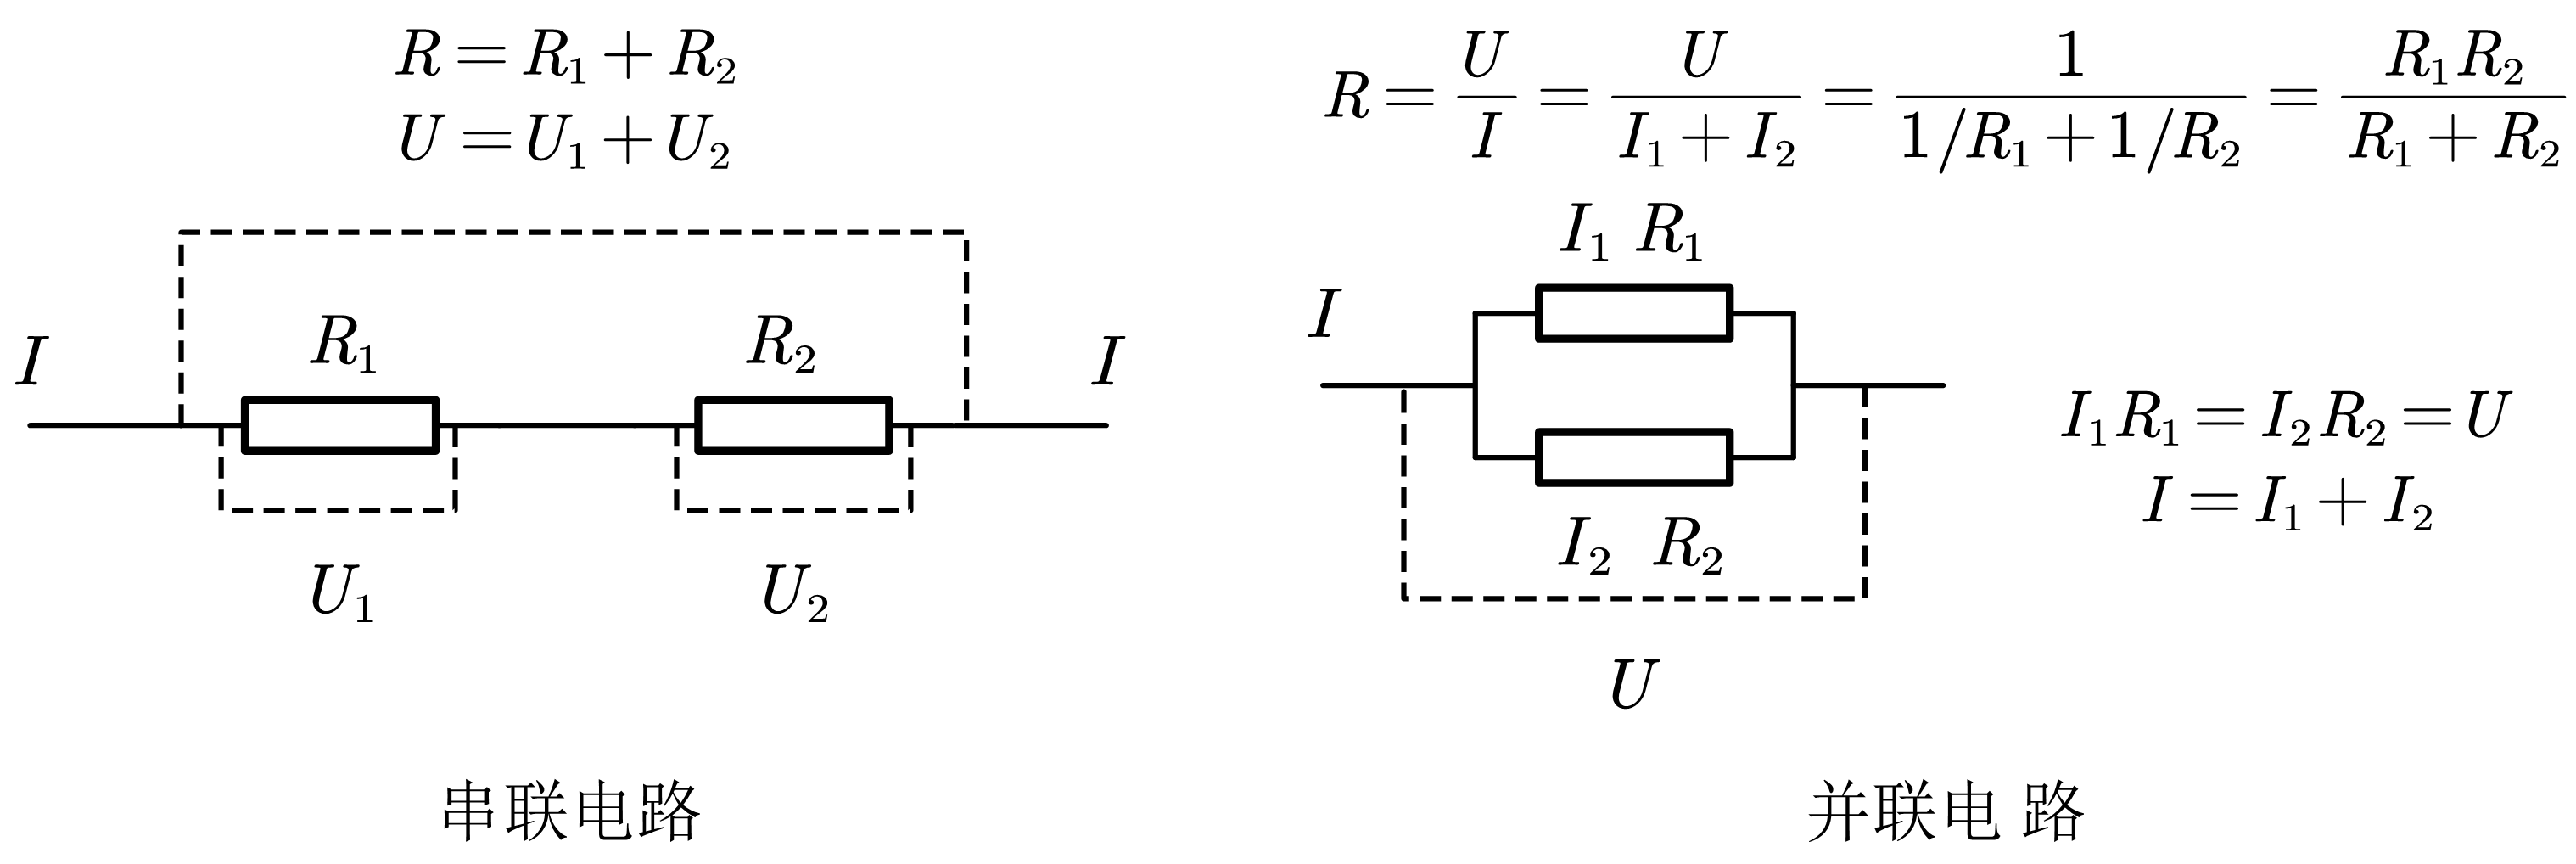
\includegraphics[width=14cm]{figure/seq-vs-parrllel-circuit.png}
\end{center}

\paragraph*{基尔霍夫定律}描述复杂电路中支路的电流与电压的关系,在每个节点处有:
\begin{empheq}{align}
\sum_{k=1}^{n}i_k&=0\mtag{基尔霍夫第一定律}\\
\sum_{j=1}^{n}v_j&=0\mtag{基尔霍夫第二定律}
\end{empheq}
当电流注入节点时,$i_k$为正,否则为负。$v_j$表示某个元件的电势差(有正负)。第一定律针对节点,也可以表达为注入某节点的电流等于流出节点的电流。第二定律针对整个闭合回路(电源也算,回路也可以是电路的一部分)。

\paragraph*{惠更斯电桥}一五电阻电路:
\begin{center}
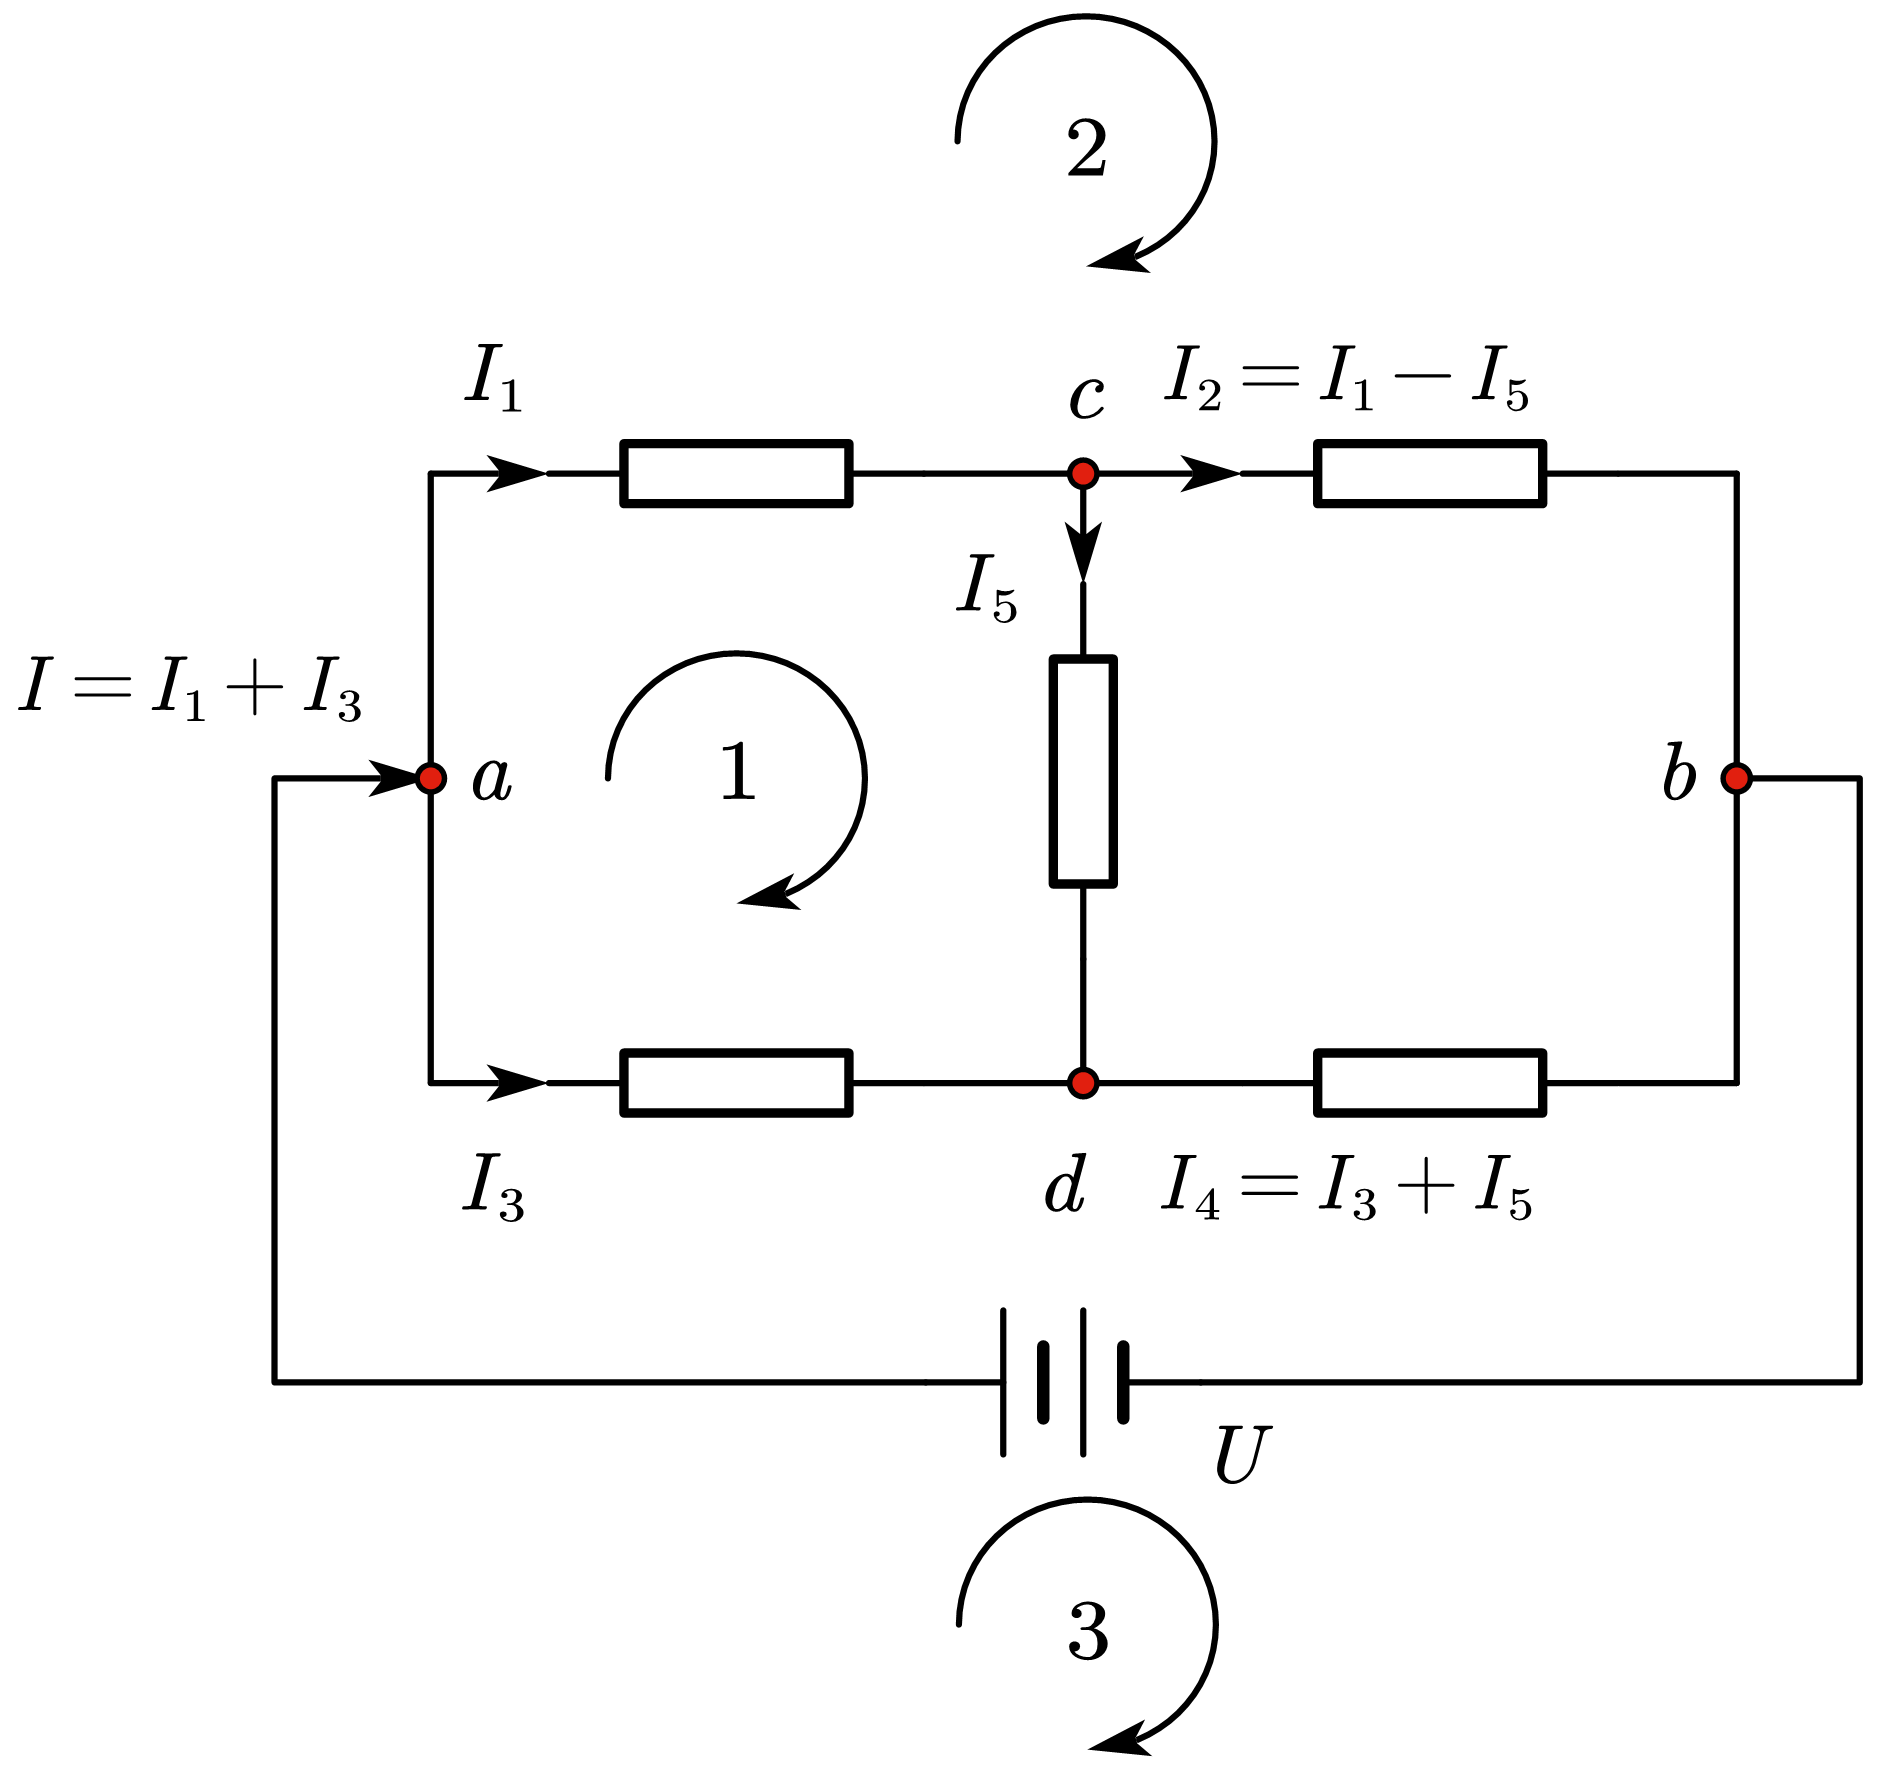
\includegraphics[width=8cm]{figure/5R-elec-bridge.png}
\end{center}
用并联与串联电路不能求解,需要使用基尔霍夫定律。
对于图示的三个回路有:
\begin{enumerate}
\item 回路1,$acda$:$I_1R_1+I_5R_5-I_3R_3=0$
\item 回路2,$acbda$:$(I_1-I_5)R_2-(I_3+I_5)R_4-I_5R_5=0$
\item 回路3,$acbUa$:$I_1R_1+(I_1-I_5)R_2-U=0$
\end{enumerate}
电流有3个,方程有3个,且为线性方程组,可以求解:
\begin{empheq}{align}
I_1&=\frac{U}{\Delta}((R_2+R_4)R_3+(R_3+R_4)R_5)\\
I_3&=\frac{U}{\Delta}((R_2+R_4)R_1+(R_1+R_2)R_5)\\
I_5&=\frac{U}{\Delta}(R_2R_3-R_1R_4)\\
\Delta &=R_1R_2(R_3+R_4)+R_3R_4(R_1+R_2)+(R_1+R_2)(R_3+R_4)R_5
\end{empheq}
可知
$$I=I_1+I_3=\frac{U}{\Delta}((R_1+R_3)(R_2+R_4)+(R_1+R_2+R_3+R_4)R_5)$$
于是$ab$间电阻为:
$$R_{ab}=\frac{U}{I}=\frac{R_1R_2(R_3+R_4)+R_3R_4(R_1+R_2)+(R_1+R_2)(R_3+R_4)R_5}{(R_1+R_3)(R_2+R_4)+(R_1+R_2+R_3+R_4)R_5}$$

\subsubsection{交流电}

\subsection{磁}
\subsubsection{磁场}
磁场可以内磁感应强度来刻画:

\paragraph*{磁感应强度Magnetic induction} 与电场强度对应,描述了磁场的大小和方程。用$\bB$表示,单位\si{\N\s\per(\coulomb\m)}=\si{\N\per(\ampere\m)},称为特斯拉,用\si{\tesla}表示。$\bB$的尤洛卡为单位正电荷以单位速度通过该点时受到的最大作用力:
$$B=\frac{F_{\max}}{qv},\quad \bm{F}=q(\bB\times\bm{v})$$

由磁感应强度衍生出:
\begin{description}
\item[磁感应通量]\label{magnetic-induction-flux} 与电通量对应:
$$\Phi_{\bB}=\iint_S\bB\cdot\dif \bm{s}$$
单位\si{\tesla\square\m},叫做韦伯,符号\si{\weber}。
\item[磁场强度] 为了方便书写而引入的符号,用$\bm{H}$表示:
$$\bm{H}=\frac{\bB}{\mu_0}-\bm{M}$$
\end{description}

\paragraph*{磁矢势}磁场是有旋无散场,即$\nabla\cdot \bB=0$,则根据向量分析的定理\ref{vec-ana-div-zero},存在$\bm{A}$,满足$\bB=\nabla \times \bm{A}$。$\bm{A}$就称为磁矢势。

\begin{description}
\item[磁矩]  考查运动电荷体系产生的磁势。记$\bar{\bA}$为平均矢势,即对时间的平均,现在它只是对坐标的函数。类似于电极矩中的定义,以$\bm{r}_i$记径矢,则磁矢势
$$\bar{\bA}=\frac{1}{c}\frac{\bar{q_i\bm{v}_i}}{|\bm{R}_0-\bm{r}_i|}$$
展开为幂级数:
$$\bar{\bA}=\inv{cR_0}\sum q\bar{\bm{v}}-\inv{c}\sum \overline{q\bm{v}\left(\bm{r}\cdot \nabla \inv{R_0}\right)}$$
对第一项
$$\sum q\bar{\bm{v}}=\overline{\odv{}{t}\sum q\bm{r}}=0$$
这是因为在一个有限范围内变化的量的导数的均值为0。还剩下一项
$$\bar{\bA}=-\inv{c}\sum \overline{q\bm{v}\left(\bm{r}\cdot \nabla \inv{R_0}\right)}=\inv{cR_0^3}\sum \overline{q\bm{v}(\bm{r}\cdot\bm{R}_0)}$$
注意到$\bm{v}=\dot{\bm{r}}$,于是
$$\sum q\bm{v}(\bm{r}\cdot\bm{R}_0)=\inv{2}\odv{}{t}\sum q\bm{r}(\bm{r}\cdot\bm{R}_0)+\inv{2}\sum q(\bm{v}(\bm{r}\cdot\bm{R}_0)-\bm{r}(\bm{v}\cdot\bm{R}_0))$$
第一项的平均也是0,则
$$\bar{\bA}=\inv{2cR_0^3}\sum\overline{q(\bm{v}(\bm{r}\cdot\bm{R}_0)-\bm{r}(\bm{v}\cdot\bm{R}_0)}$$
记
$$\bm{\mathfrak{m}}=\inv{2c}\sum q\bm{r}\times \bm{v}$$
为磁矩。此时
$$\bar{\bA}=\frac{\bar{\bm{\mathfrak{m}}}\times \bm{R}_0}{R_0^3}=\nabla \inv{R_0}\times\bar{\bm{\mathfrak{m}}}$$
这里参考$\times$的运算公式\cref{triple-cross-prod-rule}。利用磁矩可以改写磁场公式:
$$\bar{\bH}=\vcurl \bar{\bA}=\vcurl \frac{\bar{\bm{\mathfrak{m}}}\times \bm{R}_0}{R_0^3}=\bar{\bm{\mathfrak{m}}}\vdiv \frac{\bm{R}_0}{R_0^3}-(\bar{\bm{\mathfrak{m}}}\cdot\nabla)\frac{\bm{R}_0}{R_0^3}$$
由于$\vdiv \vdiv \frac{\bm{R}_0}{R_0^3}=0$,且
$$(\bar{\bm{\mathfrak{m}}}\cdot\nabla)\frac{\bm{R}_0}{R_0^3}=\frac{\bar{\bm{\mathfrak{m}}}}{R_0^3}-\frac{3\bm{R}_0(\bar{\bm{\mathfrak{m}}}\cdot\bm{R}_0)}{R_0^5}$$
因此
$$\bar{\bH}=\frac{3\bm{n}(\bar{\bm{\mathfrak{m}}}\cdot\bm{n})-\bar{\bm{\mathfrak{m}}}}{R_0^3}$$

假如电荷具有相同的荷质比,则磁矩
$$\bm{\mathfrak{m}}=\inv{2c}\sum q\bm{r}\times \bm{v}=\frac{q}{2mc}\sum m\bm{r}\times \bm{v}=\frac{q}{2mc}\sum \bm{r}\times \bm{p}=\frac{q}{2mc}\bm{M}$$
当$v\ll c$时,$\bm{p}=m\bm{v}$为动量,$\bm{M}$为角动量,参考\ref{move-rot-formulas}。即磁矩与角动量之比为常数。
\end{description}
\subsubsection{磁介质}
\paragraph*{磁导率Magnetic permeability}表征磁介质导磁性能的物理量,
\begin{empheq}{align}
\mu&=\mu_0\mu_r\\
\mu_r&=1+\chi_m
\end{empheq}
$\mu$为绝对磁导率,$\mu_0$为真空磁导率,$\mu_r$为相对磁导率。
\paragraph*{磁化}
原来不显示磁性的磁介质在外加磁场$\bB_0$的作用下显示磁性,产生附加磁场。磁化后在介质的表面或者内部会产生等效的磁化电流,磁化电流产生磁场$\bB'$,则磁介质内部的总磁场为$\bB=\bB'+\bB_0$。

描述磁化的物理量有:
\begin{description}
\item[磁化强度] 向量。描述介质磁化程度的量。用$\bm{M}$表示:
$$\bm{M}=\frac{\sum \bm{m}_{\text{分子}}}{\Delta V}$$
即单位体积内分子磁矩的的矢量和,单位\si{\ampere\per\m}。
\item[磁化率] 磁化强度$\bm{M}$与磁场强度$\bm{H}$的关系叫介质的磁化规律,比例称为磁化率,用$\chi_m$表示:
$$\bm{M}=\chi_m\bm{H}$$
\end{description}

\subsection{相互作用}
\subsubsection{受力}
\paragraph*{洛伦兹力}运动电荷在电磁场中的受力:
$$\bm{F}=q(\bE+\bm{v}\times \bB)$$
如果磁感应强度为0,或者静止,显然只受电场力。由于磁场力是垂直于运动方向的,所以磁场不做功。

\paragraph*{安培力}电流元在磁场中的受力:
$$\dif \bm{F}=I\dif\bm{l}\times\bB$$
对一段导线进行积分,可以求得整个导线在磁场中受的合力。

\paragraph*{安培定律}描述了两个电流元间的相互作用力:
$$\dif \bm{F}_{21}=\frac{\mu_0}{4\pi\varepsilon_0}\frac{I_1I_2\dif\bm{l}_2(\dif \bm{l}_1\times\bm{e}_{21})}{r_{21}^2}$$
对于两段平行导线,这个作用力是:
$$F=\frac{\mu_0}{2\pi}\frac{I_1I_2}{r^2}$$

\subsubsection{电磁感应}
\paragraph*{磁$\rightarrow$电}导体运动或者磁场变化引用的电动势。如下图所示:

\begin{center}
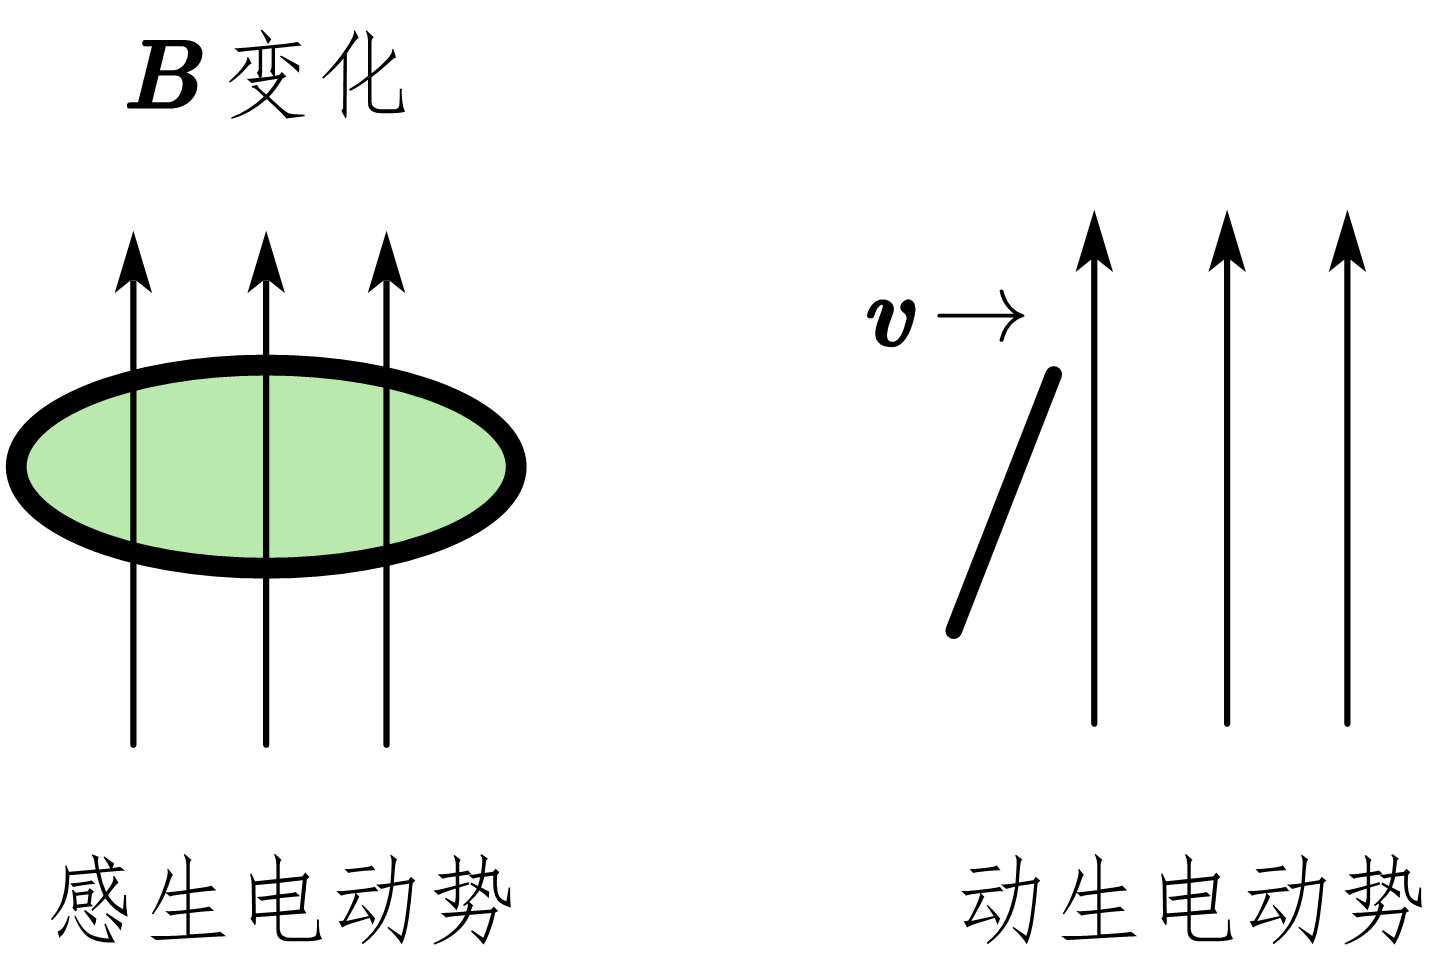
\includegraphics[width=6cm]{figure/magnetic-to-current.png}
\end{center}

\begin{description}
\item[感生电动势induced electromotive force] 导体不动,由磁场变化而引发的电动势:
$$\varepsilon =\oint_L\bE\cdot\dif\bm{l}=\oiint_S \pdv{\bB}{t}\cdot\dif \bm{s}$$

一个特殊的情形是法拉弟电磁感应:
$$\varepsilon=-\odv{\Phi_{\bB}}{t}$$
$\Phi_{\bB}$为磁感应通量\ref{magnetic-induction-flux}。
\end{description}


\paragraph*{电$\rightarrow$磁}
\begin{description}
\item[毕奥-萨伐尔定律Biot-Savart]给出了电流元激发的磁感应强度。而电流是电荷的运动。

$$\dif \bB=\frac{\mu_0}{4\pi\varepsilon_0}\frac{I\dif \bm{l}\times \bm{e}_r}{r^2}$$

$\dif\bm{l}$是电流元,$r$是电流元到点的距离,$\bm{e}_r$是电流元指向点的单位矢量。对上式积分可以求出任意形状曲线在某点处的磁感应强度。
\end{description}

\subsection{电磁波}

\subsection{电磁场的张量分析}
这部分内容主要来自朗道的《场论》,使用了相对论原理。

\subsubsection{四维矢量}
\paragraph*{事件坐标与四维径向矢量} 四维时空的一个事件的坐标记为:$(x^0,x^1,x^2,x^3)=(ct,x,y,z)$。该矢量长度的平方为$(x^0)^2-(x^1)^2-(x^2)^2-(x^3)^2$,它在四维坐标系的任意转动下不变。
\paragraph*{四维矢量的定义}如果四个量$A^0,A^1,A^2,A^3$在四维坐标系的变换下像四维径向矢量那样变换,就称为四维矢量$A^i$。在洛伦兹变换下:
\begin{empheq}{align}
A^0&=\frac{A^{'0}+V/cA^{'1}}{\sqrt{1-V^2/c^2}}\\
A^1&=\frac{A^{'1}+V/cA^{'0}}{\sqrt{1-V^2/c^2}}\\
A^2&=A^{'2}\\
A^3&=A^{'3}
\end{empheq}
同时引入$(A_0,A_1,A_2,A_3)=(A^0,-A^1,-A^2,-A^3)$。$A^i$称为四维矢量的逆变分量,$A_i$称为协变分量。

量$A^iB_i$为一个标量,类似地有$A^iA_i$,即四维矢量的长度平方。分量$A^0$称为四维矢量的时间分量,$A^1,A^2,A^3$称为空间分量。四维矢量的平方可以为正(类时矢量)、负(类空矢量)、零(类光矢量)。

在纯空间转动(不影响时间)下,三个空间分量构成一个三维矢量$\bm{A}$,此时也记
\begin{empheq}{align}\label{elect-mag-4d-vec-def}
A^i&=(A^0,\bm{A})\\
A_i&=(A^0,-\bm{A})\\
x^i&=(ct,\bm{r})\\
x_i&=(ct,-\bm{r})\\
x^ix_i&=c^2t^2-\bm{r}^2
\end{empheq}

\paragraph*{二阶四维张量}对应于矩阵。是16个量$A^{ik}$的集合,在坐标变换下像两个四维矢量分量的积那样变换。一个二阶张量的分量可以写成三种形式:协变的$A_{ik}$,逆变的$A^{ik}$,混合的$A^i_{\ k}$、$A_{\ i}^k$。

这些分量之间的变换规则是:
\begin{enumerate}
\item 升降一个空间指标时变号:$A_0^{\ 1}=A^{01},A^1_{\ 1}=-A^{11}=A_{11}$。则升降两个空间指标不变号:$A^{11}=A_{11}$。
\item 升降时间指标不变号:$A^0_{\ 0}=A^{00}=A_{00},A_{00}=A^{00},A_{01}=-A^{01}$。
\end{enumerate}

如果$A^{ik}=A^{ki}$,则称为对称张量。如果$A^{ik}=-A_{ki}$,则称为反对称张量,反对称张量的对角线元素为0。

\paragraph*{四维张量的运算}
\begin{description}
\item[缩并] $A^i_{\ i}=A^0_{\ 0}+A^2_{\ 2}+A^3_{\ 3}+A^4_{\ 4}$,这里$A^i_{\ i}=A^{\ i}_i$。
\item[]
\end{description}

\paragraph*{单位张量与度规张量}单位四维张量 $\delta^i_j$,其实就是$\delta$函数。对$\delta^i_j$升降指标得到度规张量$g^{ik},g_{ik}$,两个的分量相同,其矩阵式为$(g^{ik})=(g_{ik})=\diag([1,-1,-1,-1])$。度规张量与四维矢量的计算如下:
$g_{ik}A^k=A_i,g^{ik}A_k=A^i,A^iA_i=g_{ik}A^iA^k=g^{ik}A_iA_k$

类似地有四阶全反对称张量$e^{iklm}$,它的分量在交换任意一对指标时变号,非零分量为$\pm 1$。由其反对称性,具有相同两个指标的所有分量为0。同时约定:
\begin{empheq}{equation}
e^{0123}=1,\quad e_{0123}=-1
\end{empheq}
可知$e^{iklm}e_{iklm}=-24$。这是因为4个指标有24种排列,相同的上下标反号,则乘积-1。

\paragraph*{赝张量}赝张量在反射以外的坐标转动下都具有张量的性质。反射(坐标正负号改变,镜像对称)是特殊的,因为它不能归结为转动。


\paragraph*{四维矢量的微分}
\begin{enumerate}
\item[梯度] 标量$\varphi$的四维梯度是四维矢量:
$$\pdv{\varphi}{x^i}=(\inv{c}\pdv{\varphi}{t},\nabla \varphi)$$
这些导数是梯度四维矢量的协变分量。这是因为标量的微分 $\dif\varphi=\pdv{\varphi}{x^i}\dif x^i$,形式为两个四维矢量的标量积。
\end{enumerate}

\paragraph*{四维矢量的积分}四维空间中的积分有4种类型:
\begin{enumerate}
\item 沿四维空间中的曲线积分。积分元是线元:$\dif x^i$。
\item 沿四维空间中一个二维曲面积分。无穷小面元为一个二阶反对称张量:$\dif f^{ik}=\dif x^i\dif x^{'k}-\dif x^k \dif x^{'i}$,这里$\bx,\bx'$为两个四维矢量,$\dif f^{ik}$为两个四维矢量张成的面元在坐标面上的投影。类似地可以构造$\dif f^{ik}$的对偶张量:
$$\dif f^{*ik}=\inv{2}e^{iklm}\dif f_{lm}$$
\item 沿一个超曲面(三维流形)的积分。三个四维矢量张成的平等六面体体积的投影为:
\begin{empheq}{equation}
\dif S^{ikl}=\begin{matrix}
\dif x^i & \dif x^{'i} & \dif x^{''i}\\
\dif x^k & \dif x^{'k} & \dif x^{''k}\\
\dif x^l & \dif x^{'l} & \dif x^{''l}
\end{matrix}
\end{empheq}
使用与$\dif S^{ikl}$对偶的四维矢量$\dif S^i$更方便:
\begin{empheq}{align}
\dif S^i=-\inv{6}\dif e^{iklm}\dif S_{klm}&\quad \dif S_{klm}=e_{nklm}\dif S^n\\
\dif S^0=\dif S^{123}=\dif x\dif y\dif z,\dif S^1=\dif S^{023}
\end{empheq}

\item 沿四维体积的积分。积分元是标量:
$$\dif \Omega=\dif x^0\dif x^1\dif x^2\dif x^3=c\dif t\dif V$$
\end{enumerate}

\subsubsection{电磁场的四维势}
\paragraph*{四维势的定义}一个电磁场可以用一个四维势$A_i$表征,它的分量是坐标与时间的函数。其三维空间分量构成一个三维空间矢量$\bA(t,\bm{r})$,称为矢势;时间分量称为标势。于是:
$$A^i=(\varphi, \bA)$$

四维势的具有以下性质:
\begin{empheq}{align}
\odv{\bA}{t}=\pdv{\bA}{t}+(\bm{v}\cdot \nabla)\bA
\end{empheq}

\paragraph*{四维势与最小作用量}电磁场中电荷的作用量形式为
\begin{empheq}{align}
S&=\int_{a}^{b}-mc\dif s-\frac{q}{c}A_i\dif x^i\label{4d-elec-mag-action}\\
&=\int_{a}^{b}(-mc\dif s+\frac{q}{c}\bA\cdot\dif \bm{r}-q\varphi\dif t)\nonumber\\
&=\int_{t_0}^{t_1}\left(-mc^2\sqrt{1-v^2/c^2}+\frac{q}{c}\bA\cdot\bm{v}-q\varphi\right)\dif t\label{4d-elec-mag-charge-lag}\\
&=\int_{t_0}^{t_1} L\dif t
\end{empheq}
式\ref{4d-elec-mag-action}中的第一项与电荷自身有关,而第二项与场有关。$L$即为拉格朗日量。

\paragraph*{四维势与电场、磁场强度}根据拉格朗日方程:
\begin{empheq}{equation}
\odv{}{t}\pdv{L}{\bm{v}}=\pdv{L}{\bm{r}}
\end{empheq}
式中$L$即为\cref{4d-elec-mag-charge-lag}。上式右边:
\begin{empheq}{align}
\pdv{L}{\bm{r}}&=\frac{1}{c}\nabla (\bA\cdot\bm{v})-q\nabla \varphi\\
&=\frac{q}{c}(\bm{v}\cdot \nabla)\bA+\frac{1}{c}\bm{v}\times \vcurl \bA-q\nabla \varphi
\end{empheq}
这里用到了向量场内积的微分式\cref{div-of-inner-prod}。

拉格朗日方程左边:
$$\odv{}{t}\pdv{L}{\bm{v}}=\odv{}{t}\left(\bm{p}+\frac{q}{c}\bA\right)$$

于是有:
\begin{empheq}{equation}
\odv{\bm{p}}{t}=-\frac{q}{c}\pdv{\bA}{t}-q\nabla \varphi+\frac{q}{c}\bm{v}\times \vcurl \bA
\end{empheq}
式中第一部分(第一、二项)与速度无关,对应电场的效应;而第二部分(第三项)与速度有关,且垂直于速度,对于磁场的效应。作用于粒子第一类型的力,称为电场强度;第二类型的力,就是磁场强度。于是有:
\begin{empheq}{align}\label{elec-mag-E-H-tensor-def}
\bE&=-\inv{c}\pdv{\bA}{t}-\nabla\varphi\\
\bm{H}&=\vcurl \bA
\end{empheq}
此式给出了电场强度与磁场强度的关系。在一电磁场中,如果$\bm{H}=0,\bE\neq 0$,就是电场,反之为磁场。

这里可以看出,电磁场的四维势统一了电场与磁场。

\subsubsection{电磁场中的张量}
\paragraph*{电磁场张量}再考查式\cref{4d-elec-mag-action}的最小作用量原理:
\begin{empheq}{align}
\delta S=\delta \int_{a}^{b}-mc\dif s-\frac{q}{c}A_i\dif x^i=0
\end{empheq}
由于$\dif s=\sqrt{\dif x_i\dif x^i}$,于是
\begin{empheq}{align}
\delta S=-\int\left(mc\frac{\dif x_i\dif \delta x^i}{\dif s}+\frac{q}{c}\bA_i\dif \delta x^i+\frac{q}{c}\delta A_i\dif x^i\right)=0
\end{empheq}
取$\odv{x_i}{s}=u_i$。现在用分部积分,于是第一项为:
$$mcu\delta x^i-\int mc\delta x^i\dif u_i$$
第二项为
$$\frac{q}{c}(A_i \delta x^i-\int \delta x^i\dif A_i)$$
整理后有:
\begin{empheq}{equation}
\int \left(mc\delta x^i\dif u_i+\frac{q}{c}\delta x^i\dif A_i-\frac{q}{c}\delta A_i\dif x^i\right)-\left(mcu_i+\frac{q}{c}A_i\right)\delta x^i=0
\end{empheq}
由于边界固定,因此第二项为0。同时有:
\begin{empheq}{equation}
\delta A_i=\pdv{A_i}{x^k}\delta x^k,\quad \dif A_i=\pdv{A_i}{x^k}\dif x^k
\end{empheq}
那么:
\begin{empheq}{equation}
\int \left(mc\dif u_i\delta x^i+\frac{q}{c}\pdv{A_i}{x^k}\delta x^i\dif x^k-\frac{q}{c}\pdv{A_i}{x^k}\dif x^i\delta x^k\right)=0
\end{empheq}
现在再根据表达式:$\dif u_i=\odv{u_i}{s}\dif s,\dif x^i=u^i\dif s$,同时交换第三项的$i,k$指标,则
\begin{empheq}{equation}
\int\left(mc\odv{u_i}{s}-\frac{q}{c}\left(\pdv{A_k}{x^i}-\pdv{A_i}{x^k}\right)u^k\right)\delta x^i\dif s=0
\end{empheq}
一阶条件为:
\begin{empheq}{equation}
mc\odv{u_i}{s}-\frac{q}{c}\left(\pdv{A_k}{x^i}-\pdv{A_i}{x^k}\right)u^k=0
\end{empheq}
引入符号:
\begin{empheq}{equation}\label{elec-mag-tensor}
F_{ik}=\pdv{A_k}{x^i}-\pdv{A_i}{x^k}
\end{empheq}
反对称张量$F_{ik}$称为电磁场张量,此时运动方程为:
\begin{empheq}{equation}
mc\odv{u_i}{s}=\frac{q}{c}F^{ik}u_k
\end{empheq}
这是四维形式的电荷运动方程。

将$A_i=(\varphi, -\bA)$代入定义式\cref{elec-mag-tensor},可得
\begin{empheq}{equation}
F_{ik}=\begin{bmatrix}
0 & E_x & E_y & E_z\\
-E_x & 0 & -H_z & H_y\\
-E_y & H_z & 0 & -H_x\\
-E_z & -H_y & H_x & 0
\end{bmatrix},\quad F^{ik}=\begin{bmatrix}
0 & -E_x & -E_y & -E_z\\
E_x & 0 & -H_z & H_y\\
E_y & H_z & 0 & -H_x\\
E_z & -H_y & H_x & 0
\end{bmatrix}
\end{empheq}
也可以表示为:
\begin{empheq}{equation}
F_{ik}=(\bE,\bH),\quad F^{ik}=(-\bE,\bH)
\end{empheq}

现在来考查一下以上的$F_{ik}$是怎么计算的:
\begin{empheq}{equation}
F_{01}=\pdv{A_1}{x^0}-\pdv{A_0}{x^1}
\end{empheq}
根据四维矢量的定义\cref{elect-mag-4d-vec-def},有$x^i=(ct,\bm{r})$,于是
\begin{empheq}{align}
\pdv{A_1}{x^0}&=-\inv{c}\pdv{A_1}{t}\\
\pdv{A_0}{x^1}&=\pdv{\varphi}{x}
\end{empheq}
于是$$F_{01}=-\inv{c}\pdv{A_1}{t}-\pdv{\varphi}{x}$$
对比电场强度的张量定义式\cref{elec-mag-E-H-tensor-def},可知
$$F_{01}=E_x$$
其它类似。

\subsection{重要原理}
\subsubsection{叠加原理}
电场强度、电势、磁感应强度都是可以叠加的。这样一来,两点电荷产生的电场就是两个点电荷产生的电场的叠加。

在向量场部分\ref{vector-field},曾经指出,向量场可以作为一阶微分算子,它就是线性的。
\section{Maxwell方程组}
\subsection{Maxwell方程组的分析}
\paragraph*{真空中的Maxwell方程组与外微分}标准的Maxwell方程包含4个方程:
\begin{empheq}{align}
\vdiv \bB&=0 \label{maxwell-1}\\
\pdv{\bB}{t}+\vcurl \bE&=\bm{0}\label{maxwell-2}\\
\vdiv \bE&=4\pi\rho\label{maxwell-3}\\
\pdv{\bE}{t}-\vcurl \bB&=-4\pi\bJ\label{maxwell-4}
\end{empheq}
这里使用普朗克自然单位制\ref{planck-natural-unit}。Maxwell方程组描述了真空中电场与磁场满足的关系。

取Minkowski四维时空$\mathbb{R}^4$上的洛伦兹度量与微分形式
\begin{empheq}{equation}
\mathcal{F}=\sum_{1}^{3}E_j\dif x_j\wedge \dif t+B_1\dif x_2\wedge x_3+B_2\dif x_3\wedge x_1+B_3\dif x_1\wedge x_2
\end{empheq}
注意$\bB$的三个下标是轮换的。

则原始Maxwell方程组可以由两个方程描述:
\begin{empheq}{align}
\dif \mathcal{F}&=0\\
\dif^{\bigstar}\mathcal{F}&=4\pi\mathcal{J}^b
\end{empheq}
\cref{maxwell-1,maxwell-2}由前一个方程描述,而\cref{maxwell-3,maxwell-4}由后两个方程描述。式中
\begin{empheq}{equation}
\mathcal{J}^b=-\rho\dif t+\sum_{1}^{3}\bJ_k\dif x_k
\end{empheq}
它是一个四维电流密度(电荷-电流4矢量)
\begin{empheq}{equation}
\mathcal{J}=(\rho,\bJ)
\end{empheq}
的1-形式。

\paragraph*{存在电介质的Maxwell方程组}

\subsection{Maxwell方程组的应用}
\subsubsection{电磁场}
\paragraph*{单点电荷的电场}从\ref{maxwell-3}可以导出单点电荷的电场。以该点电荷为中心,取一个球$\Omega$,其半径为$r$,对\ref{maxwell-3}的两边在整个球上积分:
$$\int_{\Omega} \vdiv \bE\dif V=\int_{\Omega}4\pi\rho\dif V$$
根据外微分定理,对球的积分可以转换成对球面的积分,由于球的对称性,球面上所有点处场强相同,为$\bE$。则上式左边为$4\pi r^2E$。现在考虑右边,$\rho$本身是$\bx$的函数,但现在是点电荷,则在原点处的$\rho=\infty$,而在其它点,$\rho=0$,根据$\delta$函数的性质,积分应为$4\pi q$。于是$4\pi r^2 \bE =4\pi q$,于是$\bE=\frac{q}{r^2}$,注意这里用的自然单位制。

\subsubsection{电磁波}
\paragraph*{波动方程}对\cref{maxwell-2,maxwell-4}两边取$\nabla \times$,则对\cref{maxwell-2}有:
\begin{empheq}{align*}
\nabla \times \pdv{\bm{B}}{t}+(\nabla(\nabla\cdot \bE)-\nabla^2 \bE)&=0\\
\pdv{}{t}(\nabla \times\bB)-\nabla^2\bE&=0\\
\pdv{}{t}\left(\pdv{}{t}\bE+4\pi\bm{J}\right)-\Delta \bE&=0\\
\implies \pdv[order=2]{\bE}{t}-\Delta \bE&=0
\end{empheq}
倒数第二步忽略了电流$\bm{J}$。最后一个就是波动方程。类似地可以导出$\bB$的波动方程。
\section{静电磁学}
\subsection{电势与电场强度的计算}
\subsubsection{有心电荷场生成的电势}

\subsubsection{带电荷曲线生成的电势}
\paragraph*{直线段生成的电势}

\begin{example}
电荷$q$均匀分布在一段长为$2l$的线段上,将它放在$x$轴上,其中心与原点重合,求它生成的电势。
\end{example}
\begin{solution}
在$x$轴上距原点中心$s$处的线元$\dif s$的电荷为$\dif q=\frac{q}{2l}\dif s$,它产生的电势为:
$$\dif \varphi(x,y,z)=k\frac{dq}{r}=k\frac{q}{2l}\frac{\dif s}{\sqrt{(x-s)^2+y^2+z^2}}$$
于是整个线段产生电势为积分:
\begin{empheq}{align*}
\varphi(x,y,z)&=k\frac{q}{2l}\int_{-l}^l\frac{\dif s}{\sqrt{(x-s)^2+y^2+z^2}}\\
&=k\frac{q}{2l}\ln\frac{\sqrt{(x+l)^2+y^2+z^2}+x+l}{\sqrt{(x-l)^2+y^2+z^2}+x-l}
\end{empheq}

另一方面,假定把这条线段放在与$x$轴平行的方向,其中心为$(x_0,y_0,z_0)$。则现在的积分为:
\begin{empheq}{align*}
\varphi(x,y,z)&=k\frac{q}{2l}\int_{-l}^l\frac{\dif s}{\sqrt{(x-s-x_0)^2+(y-y_0)^2+(z-z_0)^2}}\\
&=k\frac{q}{2l}\ln\frac{\sqrt{(x+l-x_0)^2+(y-y_0)^2+(z-z_0)^2}+x+l-x_0}{\sqrt{(x-l-x_0)^2+(y-y_0)^2+(z-z_0)^2}+x-l-x_0}
\end{empheq}

假设线段是二维的,则
$$\varphi(x,y)=k\frac{q}{2l}\ln\frac{\sqrt{(x+l)^2+y^2}+x+l}{\sqrt{(x-l)^2+y^2}+x-l}=k\frac{q}{2l}\ln\left(1+\frac{2l+\sqrt{(x+l)^2+y^2}-\sqrt{(x-l)^2+y^2}}{\sqrt{(x-l)^2+y^2}+x-l}\right)$$
考虑$\frac{2l+\sqrt{(x+l)^2+y^2}-\sqrt{(x-l)^2+y^2}}{\sqrt{(x-l)^2+y^2}+x-l}$这一项,由于分母中包含一个额外的$x$项,而在其它项中$x,y$大致是对称的,因此$x$的变动的影响大概率要略小于$y$的影响,所以平行板之间的电场强度近似于平行于$y$轴,但不是精确地平行。

现在计算场强:
\begin{empheq}{align}
E_x=-\pdv{\varphi}{x}&=\frac{1}{\sqrt{(x-l)^2+y^2}}-\inv{\sqrt{(x+l)^2+y^2}}\\
E_y=-\pdv{\varphi}{y}&=\frac{y}{\sqrt{(x-l)^2+y^2}\left(\sqrt{(x-l)^2+y^2}+x-l\right)}\\
&\quad -\frac{y}{\sqrt{(x+l)^2+y^2}  \left(\sqrt{(x+l)^2+y^2}+x+l\right)}
\end{empheq}


假设$l\rightarrow\infty,\frac{q}{2l}=\rho_0$,现在计算一下极限,对于$E_x$,相当于$\infty-\infty$,不定,需要计算一下:
\begin{empheq}{align}
\lim_{l\rightarrow\infty} E_x&=k\rho_0\lim_{l\rightarrow\infty}\frac{\sqrt{(x+l)^2+y^2}-\sqrt{(x-l)^2+y^2}}{\sqrt{(x+l)^2+y^2}\sqrt{(x-l)^2+y^2}}\\
&=k\rho_0\lim_{l\rightarrow\infty}\frac{(x+l)\left(\sqrt{1+\frac{y^2}{(x+l)^2}}-\sqrt{1+\frac{y^2-4lx}{(x+l)^2}}\right)}{\sqrt{(x+l)^2+y^2}\sqrt{(x-l)^2+y^2}}\\
&=k\rho_0\lim_{l\rightarrow\infty}\frac{(x+l)\left(\sqrt{1+\frac{y^2}{(x+l)^2}}-\sqrt{1+\frac{y^2-4lx}{(x+l)^2}}\right)}{\sqrt{(x+l)^2+y^2}\sqrt{(x-l)^2+y^2}}\\
&=k\rho_0\lim_{l\rightarrow\infty}\frac{(x+l)\frac{2lx}{(x+l)^2}}{\sqrt{(x+l)^2+y^2}\sqrt{(x-l)^2+y^2}}\\
&=0
\end{empheq}
现在考虑$\lim_{l\rightarrow\infty}E_y$,显然第二项是0,第一项的分母是$\infty\times 0$,不定,需要考虑第一项:
\begin{empheq}{align}
\lim_{l\rightarrow\infty}E_y&=k\rho_0\lim_{l\rightarrow\infty} \frac{y}{\sqrt{(x-l)^2+y^2}\left(\sqrt{(x-l)^2+y^2}+x-l\right)}\\
&=k\rho_0\lim_{l\rightarrow\infty} \frac{y}{\sqrt{(l-x)^2+y^2}\left(\sqrt{(l-x)^2+y^2}-(l-x)\right)}\\
&=k\rho_0\lim_{l\rightarrow\infty}\inv{y}\frac{\sqrt{(l-x)^2+y^2}+(l-x)}{\sqrt{(l-x)^2+y^2}}\\
&=k\rho_0\lim_{l\rightarrow\infty}\inv{y}\left(1+\frac{l-x}{\sqrt{(l-x)^2+y^2}}\right)\\
&=\frac{2k\rho_0}{y}
\end{empheq}
可见对于无穷长的线段,$x$方向场强就是0,而$y$方向不是,于是场强平行于y轴。

也可以直接考虑无穷范围的积分:
\begin{empheq}{align}
\varphi(x,y)&=\int_{-\infty}^{\infty}\frac{k\rho_0\dif s}{\sqrt{(x-s)^2+y^2}}\\
&=\int_{-\infty}^{\infty}\frac{k\rho_0\dif u}{\sqrt{u^2+y^2}}
\end{empheq}
则
\begin{empheq}{align}
E_y=-\pdv{\varphi}{y}=\int_{-\infty}^{\infty}\frac{k\rho_0 y\dif u}{\sqrt{u^2+y^2}}=\frac{2k\rho_0}{y}
\end{empheq}
与此前的结果相同。

如果是三维的,则积分与场强为
\begin{empheq}{align}
\varphi(x,y,z)&=\int_{-\infty}^{\infty}\frac{k\rho_0\dif s}{\sqrt{(x-s)^2+y^2+z^2}}\\
&=\int_{-\infty}^{\infty}\frac{k\rho_0\dif u}{\sqrt{u^2+y^2+z^2}}\\
E_x&=0\\
E_y=-\pdv{\varphi}{y}&=\frac{2k\rho_0 y}{y^2+z^2}\\
E_z=-\pdv{\varphi}{z}&=\frac{2k\rho_0 z}{y^2+z^2}
\end{empheq}
场强平行于$yz$平面(即$x$方向的分量为0),由$x$轴均匀指向外围。
\end{solution}

\paragraph*{圆锥底面圆周在顶点生成的电场}
\begin{example}\label{elec-field-from-circle-in-vertex}
现在有一个圆锥,底面半径为$r$,高度为$h$。底面圆周上均匀分布有电荷量$Q$,求圆周在顶点生成的电场强度。
\end{example}
\begin{solution}
直接在圆周上积分,水平方向的场强可以直接抵消,只需要考虑竖直方向:
\begin{empheq}{align}
\int_L \frac{kQ}{2\pi r(r^2+h^2)}\cos\theta\dif s=\int_L \frac{kQ}{2\pi r(r^2+h^2)^2}\frac{h}{\sqrt{r^2+h^2}}\dif s=\frac{kQh}{(r^2+h^2)^{\frac{3}{2}}}
\end{empheq}
上式中$\frac{Q}{2\pi r}$是密度$\rho$,$\rho\dif s$就是线元的电荷量。$\cos\theta$就是竖直方向与径矢的夹角。

另一方面也可以从电势的角度考虑:
\begin{empheq}{align}
\varphi=\int_L \frac{kQ}{2\pi r\sqrt{r^2+h^2}}\dif s =\frac{kQ}{\sqrt{r^2+h^2}}
\end{empheq}
由电势计算$z$方向(或$h$方向)的场强为:
$$E_z=-\varphi_h=\frac{kQh}{(r^2+h^2)^{\frac{3}{2}}}$$
显然两者结果一致。

由于电势的结果中不显含$x,y$,所以不能从此处的电势中得到这两个方向的场强。
\end{solution}

\paragraph*{圆周在任意点生成的电场}
\begin{example}
与上一个例子类似,现在计算底面圆周在任意点生成的电场强度。
\end{example}
\begin{solution}
把圆周放在$xy$平面上,圆心与原点重合,顶点在$z$轴上。

需要用电势进行计算:
\begin{empheq}{align}
\varphi(x,y,z)&=\int_L \frac{kQ}{2\pi rR(s)}\dif s \\
&=\int_{0}^{2\pi} \frac{kQ}{2\pi r\sqrt{(x-r\cos\theta)^2+(y-r\sin\theta)^2+z^2}}r\dif \theta
\end{empheq}
这个积分应该是没有解析解的。但可以用来考虑$x,y$方向的场强,利用积分下求导:
\begin{empheq}{align}
E_x(x,y,z)=-\pdv{\varphi(x,y,z)}{x}&=\int_{0}^{2\pi} \frac{kQ}{2\pi r\sqrt{(x-r\cos\theta)^2+(y-r\sin\theta)^2+z^2}}r\dif \theta\\
&=\int_{0}^{2\pi} \frac{kQ(r-\cos\theta)}{2\pi r\left((x-r\cos\theta)^2+(y-r\sin\theta)^2+z^2\right)^{3/2}}r\dif \theta
\end{empheq}
令$x=y=0$,则可知$z$轴上任意点处:
\begin{empheq}{align}
E_x(0,0,z)&=\int_{0}^{2\pi} \frac{-kQr\cos\theta}{2\pi r\left(r^2+z^2\right)^{3/2}}r\dif \theta=0
\end{empheq}
即$z$轴上$x$方向的场强为0,易知$y$方向也是。

$z$由上$z$方向的场强也可以由类似的方法得到:
\begin{empheq}{align}
E_z(0,0,z)&=\int_{0}^{2\pi} \frac{kQz}{2\pi r\left(r^2+z^2\right)^{3/2}}r\dif \theta= \frac{kQz}{\left(r^2+z^2\right)^{3/2}}
\end{empheq}
与上一例计算结果一致。
\end{solution}

\subsubsection{带电荷曲面生成的电势}
\paragraph*{无限大平面生成的场强}
\begin{example}
给定一个无限大的平面,面上任意点处的电荷密度为$\rho$,求该平面在任意点处生成的场强。
\end{example}
\begin{solution}
由于对称性,水平方向的场强可以抵消,只剩下$z$方向的场强。可以利用之前计算圆锥场强的结果,把平面分成无限个圆环,圆环的中心就是目标点在平面上的投影。每个圆环的半径为$r$,而宽度为$\dif r$。一个圆环在目标点处生成的场强为
$$\frac{k2\pi r \rho z}{(r^2+h^2)^{3/2}}\dif r$$
对$r$积分:
\begin{empheq}{align}
\int_{0}^{\infty}\frac{k2\pi r \rho z}{(r^2+z^2)^{3/2}}\dif r=2k\pi\rho
\end{empheq}
所以这是一个匀强电场。

能否从电势的角度出发进行计算呢?积分
$$\varphi(x,y,z)=\iint_{\Sigma} \frac{k\rho}{R(S)}\dif S$$
$\Sigma$为$x,y$平面,设为$u-v$平面,于是原积分转换为:
\begin{empheq}{align}
\varphi(x,y,z)&=\int_{-\infty}^{\infty}\int_{-\infty}^{\infty} \frac{k\rho}{\sqrt{(x-u)^2+(y-v)^2+z^2}}\dif u\dif v\\
\xRightarrow{\text{平移}}&=\int_{-\infty}^{\infty}\int_{-\infty}^{\infty} \frac{k\rho}{\sqrt{u_1^2+v_1^2+z^2}}\dif u_1\dif v_1\\
\xRightarrow{\text{极坐标}}&=\int_0^{2\pi}\dif\theta\int_{0}^{\infty}\frac{k\rho}{\sqrt{r^2+z^2}}r\dif r
\end{empheq}
注意最后这个积分是无穷大的,它不显含$x,y$,所以$E_x,E_y$必然为0。在\ref{elec-field-from-circle-in-vertex}中计算圆周的电势时,我们算出的电势中也不含$x,y$,但并不能得到$x,y$方向的场强为0,因为那里相当于只考虑点投影恰好为原点的情况,是直接从极坐标开始计算,没有进行平移坐标系这一步,所以不完整。

现在考虑$z$方向的场强:
$$E_z=-\pdv{\varphi}{z}=2\pi \int_{0}^{\infty}\frac{k\rho z}{(r^2+z^2)^{3/2}}\dif r=\sgn(z)2k\pi\rho$$

也得到了匀强电场的结论。这里$\sgn(z)$是表示平面上下的方向。
\end{solution}
\section{电磁感应}

\section{粒子与电磁场的相互作用}

\section{电磁波的传播}
\subsection{干涉}

\section{电磁辐射}


\section{电路}
\subsection{电路原理}


\subsection{电路器件}
这一部分内容主要结合Matlab中Simulink的电路元件,网址:\href{}{text}。

\subsection{传输线}
\subsubsection{基本方程}


